\section{Results \& Discussion}

\subsection*{Comparative Genomics Analysis}
\addcontentsline{toc}{subsection}{Comparative Genomics Analysis}

\normalsize

To identify genes tracing back to the last common ancestors of archaea (LACA) and bacteria (LBCA), we started from 85,205 genomes, each one the representative of species clusters, as defined by the Genome Taxonomy Database (GTDB) \cite{parks2018, parks2020, parks2022, rinke2021}. 

Since gnome completeness can lead to false-positive ortholog and erroneous species phylogeny inference \cite{kuzniar2008}, we filtered the genomes based on completeness and contamination cutoffs of $\geq$ 90\% and $\leq$ 5\%, respectively. With this approach we wanted to ensure that phylogenetic relationships and ancestral genome reconstruction would be as accurate as possible. This resulted in 52,614 high-quality (HQ) genomes, 1,785 archaeal and 50,829 bacterial, spanning 16 archaeal and 150 bacterial phyla. 

To evaluate the effect of taxon sampling and dataset size on ancestral gene content inference, we constructed eight genomic datasets of various sizes (16-1139 genomes). These span the phylum, class, order, family, and genus taxonomic levels for archaea, and at the phylum, class, and order taxonomic levels for bacteria. Dataset sizes can be found in Table \ref{gtdb_stats_no}. Even though increasing taxon sampling has been shown to improve phylogenetic accuracy, taxon evenness markedly affects tree topology \cite{graybeal1998, martinez-gutierrez2021}. To capture, therefore, the full extant phylogenetic diversity and keep the taxon sampling even and unbiased while rendering the largest of our analyses computationally tractable, we selected a single genome for each taxon, per genomic dataset/taxonomic rank in our study.

One of the primary concerns regarding the phylogenetic aspect of our analysis was its reproducibility. To review the robustness of random taxon sampling, we performed our analysis for three separately produced datasets both for the phylum and class taxonomic levels of archaea. Figure \ref{orthofinder_stats_figure}A shows the average percentage of genes assigned to orthogroups (OGs) for the two aforementioned triplicate runs, while \ref{orthofinder_stats_figure}C depicts the mean percentage of gene assignment in OGs for each of the archaea datasets. This statistic can act as a first-level quality control of an OrthoFinder (OF) analysis. A below 80\% mean assignment of genes in OGs indicates that important orthology relationships for some remaining genes are missing, likely due to poor species sampling \cite{emms2015}. Even though the number of included-in-the-analysis genomes approximately doubles per taxonomic level, the gene assignment percentage only slightly increases. The increase is justified because, as taxonomic levels become narrower, genetic distances between species decrease, allowing state-of-the-art algorithms to cluster a larger number of genes and capture in depth their phylogenetic relationships.

On a first assessment, analyzing 51 archaeal genomes at the class taxonomic level seems sufficient to capture the orthology relationships of protein-encoding genes, with over 80\% of genes assigned to OGs. However, this statistic represents the average gene assignment across all species in the dataset, masking in-group variance that is critical for analysis interpretation. Even with an average assignment above 80\%, some species may still be underrepresented in the OGs. To address this, we converted the percentage of genes assigned in OGs per species to a binary classification, where species with less than 80\% gene assignment were designated a "poorly sampled" status and given a value equal to one, while the rest were given a value of zero. The normalized distribution of poorly sampled taxa for each taxonomic level analysis can be seen in Figure \ref{orthofinder_stats_figure}D. Normalization was performed by dividing the number of poorly sampled species by the total number of species included in each respective analysis. Since the dataset sizes of the archaeal taxonomic levels vary by 1.56 orders of magnitude, this normalization allows for a direct comparison of the datasets.

A closer inspection of the statistics for individual taxa (Figure \ref{orthofinder_stats_figure}D and \ref{orthofinder_stats_figure}E) revealed that the percentage of poorly sampled genomes dropped below 5\% only at the family level (\ref{orthofinder_stats_figure}D). Interestingly, even though genomes belonging to particular phyla appear to be consistently categorized as "poorly sampled", this behavior cannot be linked to the number of species belonging to the same taxon. The Thermoproteota phylum, for example, has the highest count of "poorly sampled" species across all datasets, yet is the second richest archaeal phylum. Nanoarchaeota, on the other hand, whose genes are also consistently left out of OGs, comprise only of 4 species (Figure \ref{orthofinder_stats_figure}F). One has to take into account that species distribution remains uneven throughout the taxonomic levels, with some classes, orders, families, and genera that belong to the same phylum enriched more than others. This result is intriguing, because would expect richer phyla to have a higher assignment of genes to OGs in narrower taxonomic levels (e.g. going from phyla to classes) with the decrease in genetic distance between species as datasets grow, and taxonomic levels become narrower.  

\begin{figure}[htpb]
    \centering
    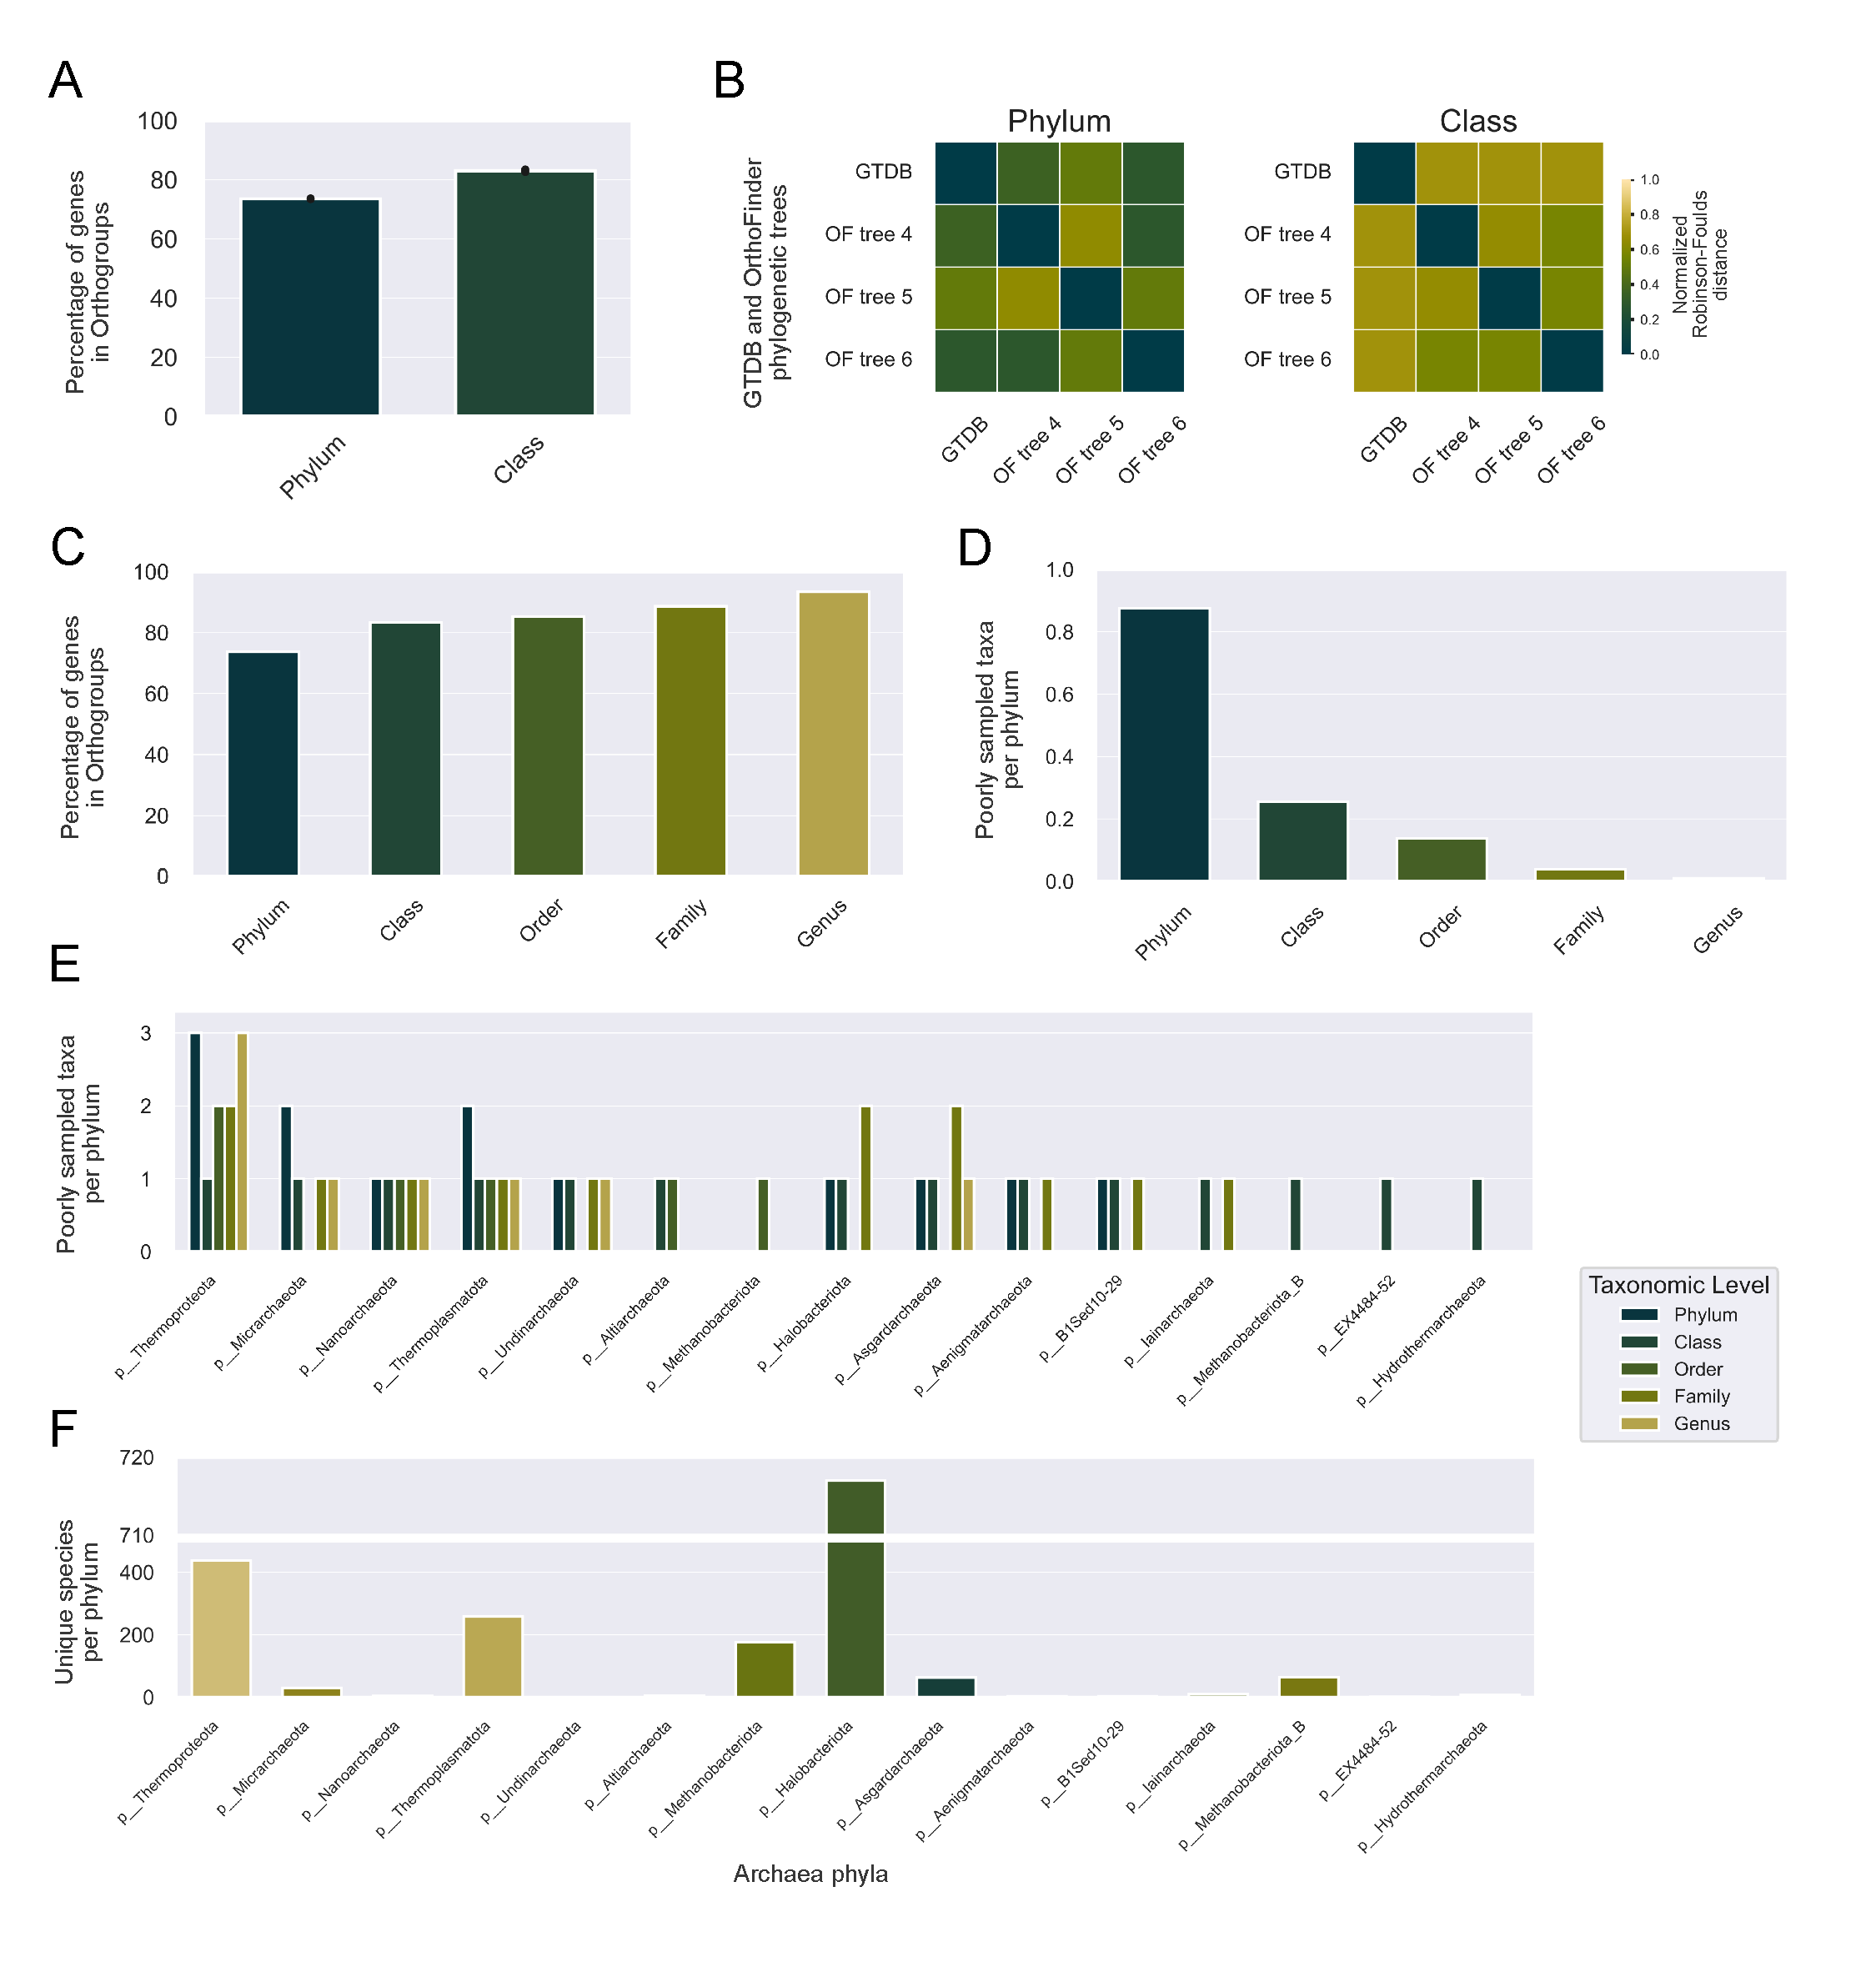
\includegraphics[width=0.97\textwidth]{fig2/fig2.pdf}
    \caption{Comparative genomics statistics of phylogenetic OrthoFinder (OF) analysis. (A) Shows the average percentage of genes assigned to OGs from three distinct datasets run by OF, for the taxonomic levels of phylum and class for archaea. (B) Presents the Robinson-Foulds (RF) distance between the trees generated by OF as part of the aforementioned analyses, as well as their RF from the GTDB archaeal tree. Since multiple datasets were generated for some of the same taxonomic levels (archaea phylum and class levels), they were assigned distinct numbers to differentiate them. These numbers appear at the heatmap axes labels. (C) Compares the percentage of genes assigned in OGs for every archaeal taxonomic level. (D) Presents the normalized distribution of poorly sampled taxa for each taxonomic level analysis. (E) Detailed distribution of poorly sampled taxa for each taxonomic level analysis, per phylum, and (F) the number of unique species per phylum taxon.}
    \label{orthofinder_stats_figure}
\end{figure}   

An initial comparison of the species trees produced by OF's STAG \cite{emms2018} and STRIDE \cite{emms2017} en-suite algorithms in Dendroscope \cite{huson2012} (found in Appendix Figures \ref{phylum_trees_all}) exposes unique tree topologies. Because of the significant missing gene orthology relationships at the phylum and class level, this does not come as a surprise. The more surprising finding comes with calculating the Robinson-Foulds (RF) distance, a direct measure of phylogenetic tree similarity. RF calculates the number of nodes that are dissimilar between the phylogenetic trees under comparison, with lower values indicating a higher similarity degree. Although the comparative genomics statistics suggest that class-level analyses encompass orthology relationships more broadly, the three species trees inferred by OF are more dissimilar both to each other and to the GTDB tree compared to the three species trees inferred for the phyla datasets (Figure \ref{orthofinder_stats_figure}B). This could be rationalized by the fact that a smaller phylum dataset with longer genetic distances would be more likely to produce the same species tree topology. Nonetheless, it raises concerns about algorithms such as STRIDE using all genes, rather than only highly conserved ones, to infer a species tree. As Martinez-Gutierrez and Aylward \cite{martinez-gutierrez2021} have pointed out, \textit{"more genes and genomes do not necessarily improve phylogenetic accuracy"}. In light of this and considering our varying dataset sizes, we have selected the GTDB domain-specific species trees for our downstream analysis.



\subsection*{Inferring ancestral genomes}
\addcontentsline{toc}{subsection}{Inferring ancestral genomes}

We wanted to utilize the full potential of the genomic data at hand for reconstructing ancestral metabolic networks, and avoid simplified approaches such as phylogenetic presence/absence profiles \cite{kreimer2008} or those using near-universal gene family distribution as filtering criteria \cite{xavier2021}. We therefore performed our phylogenetic analysis with OF \cite{emms2019, emms2015}, a comprehensive platform for comparative genomics that provides a standardized, accurate, fast, and scalable orthology inference approach. 

The relationship between the number of each ancestor's descendants and ancestral genome size can be seen in Figure \ref{node_descendants_genomesize}. The number of descendants for node zero is a direct representation of the respective dataset size, as all descendants are utilized to infer its gene content. Leaf parents---nodes that are directly above the tree leaves, where the genomes used for the phylogenetic analysis are located---like nodes 3, 5, 10, 11, 12, 13, on the other hand, tend to have the smallest number of descendants. These relationships can be seen in the phylum-level tree topology of Figure \ref{node_descendants_genomesize}B.

\begin{figure}[H]
    \centering
    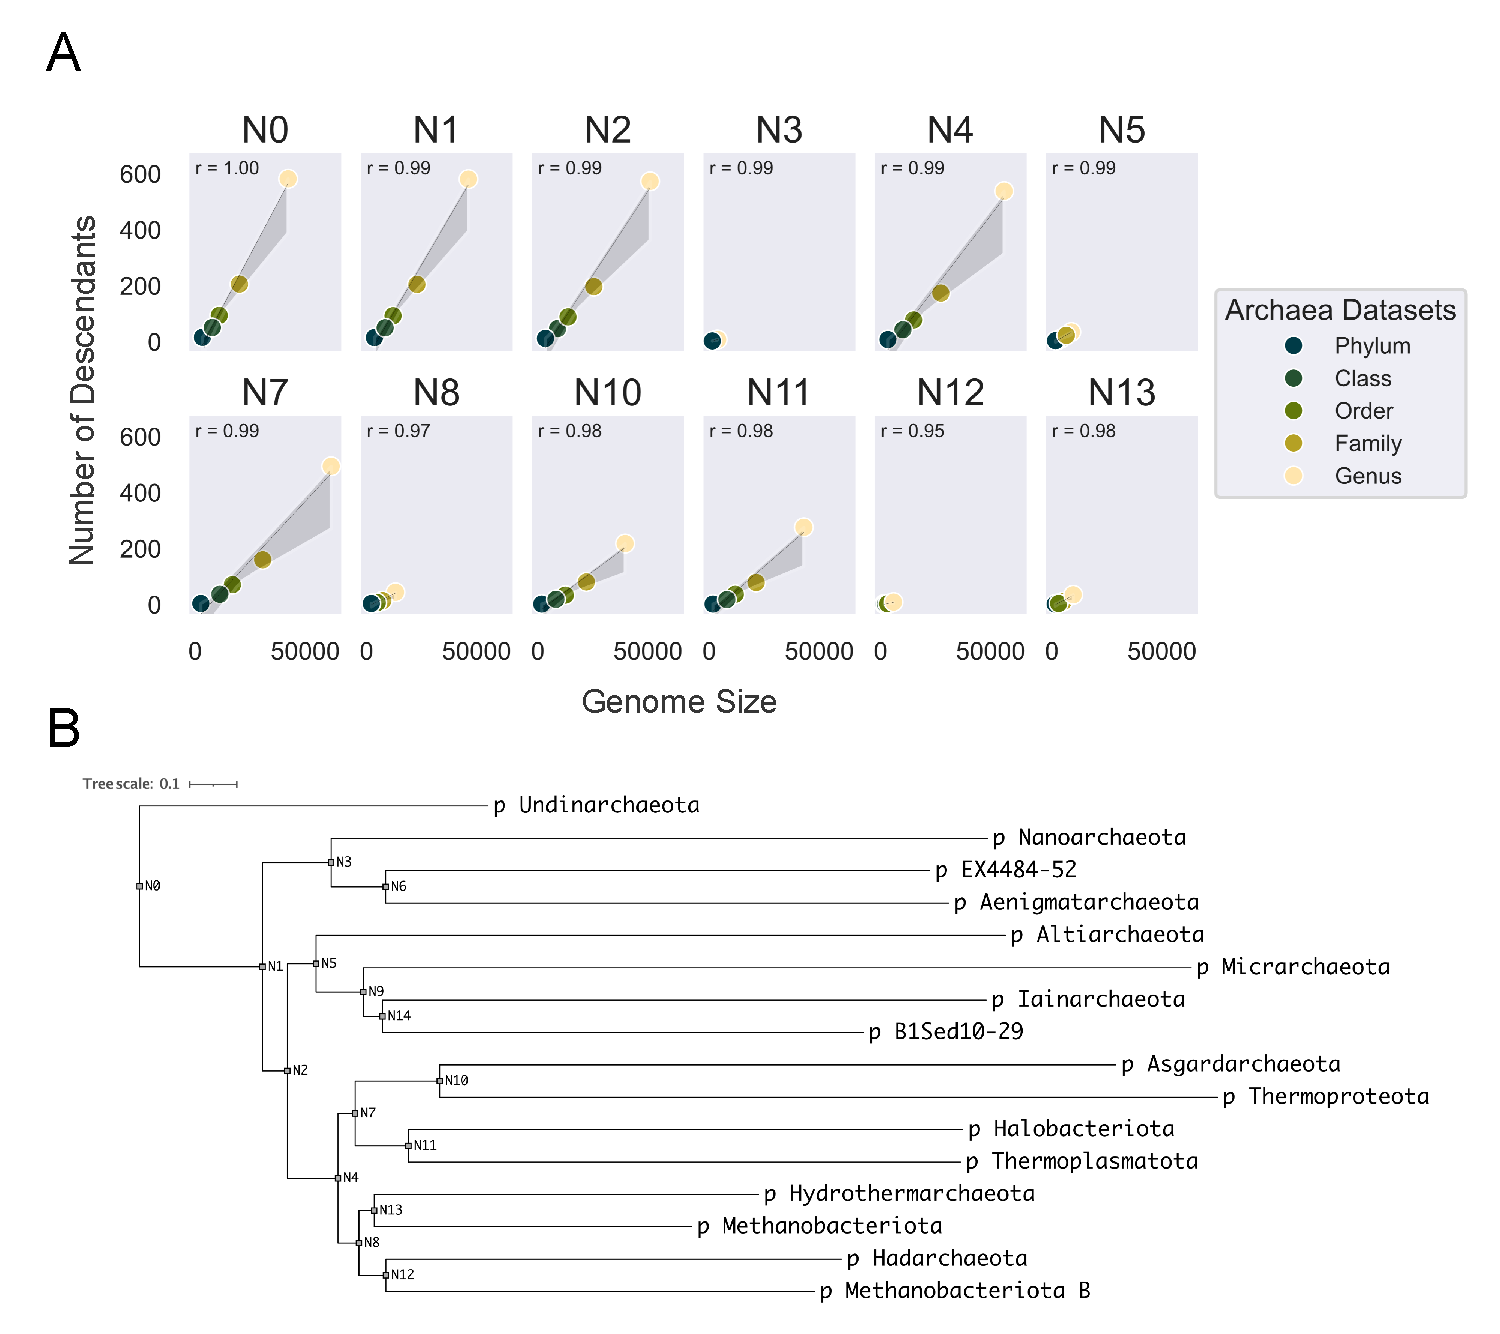
\includegraphics[width=0.95\textwidth]{fig1/fig1v2.pdf}
    \caption{Relationship between genome size and number of node descendants. (A) Shows the number of descendants of each node as a function of the inferred ancestral genome sizes, for all taxonomic levels of the archaea datasets. Colors are assigned to the five taxonomic levels, and turn lighter with narrower taxonomies. (B) Depicts the position of the nodes in the GTDB species tree, as well as their descendants. The phylum-level GTDB pruned tree has been used for simplification purposes. }
    \label{node_descendants_genomesize}
\end{figure}   

Of interest here is the uneven addition of new taxa to various tree clades when enlarging the datasets by performing the analysis at narrower taxonomic levels. Some clades experience rapid enrichment, while others remain with few taxa. This unevenness could be a direct reflection of field sampling assembly bias, but is more likely attributed to the culturability of specific taxa; genomic data originated from cultured microorganisms are of higher quality compared to metagenome-assembled genomes. For example, nodes 3 and 5, which represent a superphylum-level clade called DPANN, archaea with extremely small genome sizes and few cultured members \cite{dombrowski2019, dombrowski2020}, have very few descendants in every taxonomic-level dataset. What stands out the most, however, in Figure \ref{node_descendants_genomesize}A, is the strong positive correlation between the inferred ancestral genome size and the number of descendants/initial sampling size, with a Pearson correlation coefficient close to 1 for all nodes. 

This linear relationship can be attributed to the Duplication-Loss-Coalescence (DLC) parsimonious model for gene trees-species tree reconciliation OF utilizes. This model does not take into account horizontal gene transfer (HGT) events, and is known to overestimate gene content in ancestral genomes \cite{doolittle2003}. HGT, however, is not only omnipresent in prokaryotic evolution, but necessary for it \cite{ochman2000}. Especially when considering that any ancestral gene content reconstruction is necessarily incomplete, as the extinct gene families cannot be accounted for, it seems unreasonable that an ancient, last common ancestor would have the metabolic versatility of the entire modern biosphere. 

Despite this, the DLC model and the inferred ancestral genomes of this study may not be as unrealistic as they seem. While HGT events do exist, excluding them from evolutionary analyses and ancient genome inference might provide different insights. This approach might not point to a single ancient microorganism, as per the hypothesis surrounding LUCA's existence, but rather to a microbial community from which the modern biosphere eventually evolved. As there is still much to learn about the mechanics of evolution, it is still beneficial to consider the biosphere-level ancient genomes inferred here.

Another model, the Duplication-Transfer-Loss (DTL) model, which accounts for HGT, is able to mitigate the tendency to infer unrealistically large ancestral genomes, which get bigger with each added genome in the absence of HGT \cite{doolittle2003}. We therefore plan to redo our analysis by employing the DTL model, which has been shown to be more realistic and robust to gene tree uncertainty \cite{szollosi2013, szollosi2015}.

\subsection*{Ancestral Genome Functional Annotation}
\addcontentsline{toc}{subsection}{Ancestral Genome Functional Annotation}

For the metabolic network reconstruction of the ancestral genomes, we functionally annotated a single sequence for each of the OGs inferred to be present in the respective ancestor node. We based this decision on the rationale that an OG comprises genes that have descended from a single gene in the last common ancestor (LCA) of a group of species, and that sequences within the same OG are evolutionarily closer to each other than to sequences outside of that OG. Yet, the OGs OrthoFinder infers include both orthologs and paralogs, and functional annotation is known to be most reliable when based on orthologs, as they are expected to retain function more often than paralogs \cite{gabaldon2013a}.

To assess the impact of choosing an OG representative sequence on functional annotation, we compared the functional annotations of the first sequence within each OG against the medoid sequence of the same OG (Figure \ref{waffleplot}). The medoid sequence is the sequence with the shortest genetic distance to all other sequences in the OG, and is therefore considered a better representative of the OG than the first---essentially a random---sequence. Since OF solves the gene length bias in orthogroup inference---which tends to cluster sequences of similar length together---the produced OGs include sequences of varying lengths. It may therefore be beneficial to perform a multiple sequence alignment for each OG in the future, before choosing a representative sequence for functional annotation. Even though we do not check here for the length of the representative sequence relative to the median sequence length of an OG, there may be a selection bias towards lengths that are more common in the OG, which is also not necessarily erroneous. 

Figure \ref{waffleplot} presents the comparison statistics from the functional annotation of two sequences belonging to the same OG in the form of a waffle plot. The dataset used for this part of the study is the phylum-level archaeal dataset run against the Archaea (2157) eggNOG v5 database. EggNOG-mapper takes the protein sequences we provide and performs functional annotation after sequence alignment against the selected database, based on the best hit. Out of 2849 OGs, the first and medoid sequences differed for 68\%, were the same for 26\%, and were individual hits for 6\% (Fig. \ref{waffleplot} orange). Individual hits mean that eggNOG-mapper found a match in the database for only one of the two sequences.

\begin{figure}[H]
    \centering
    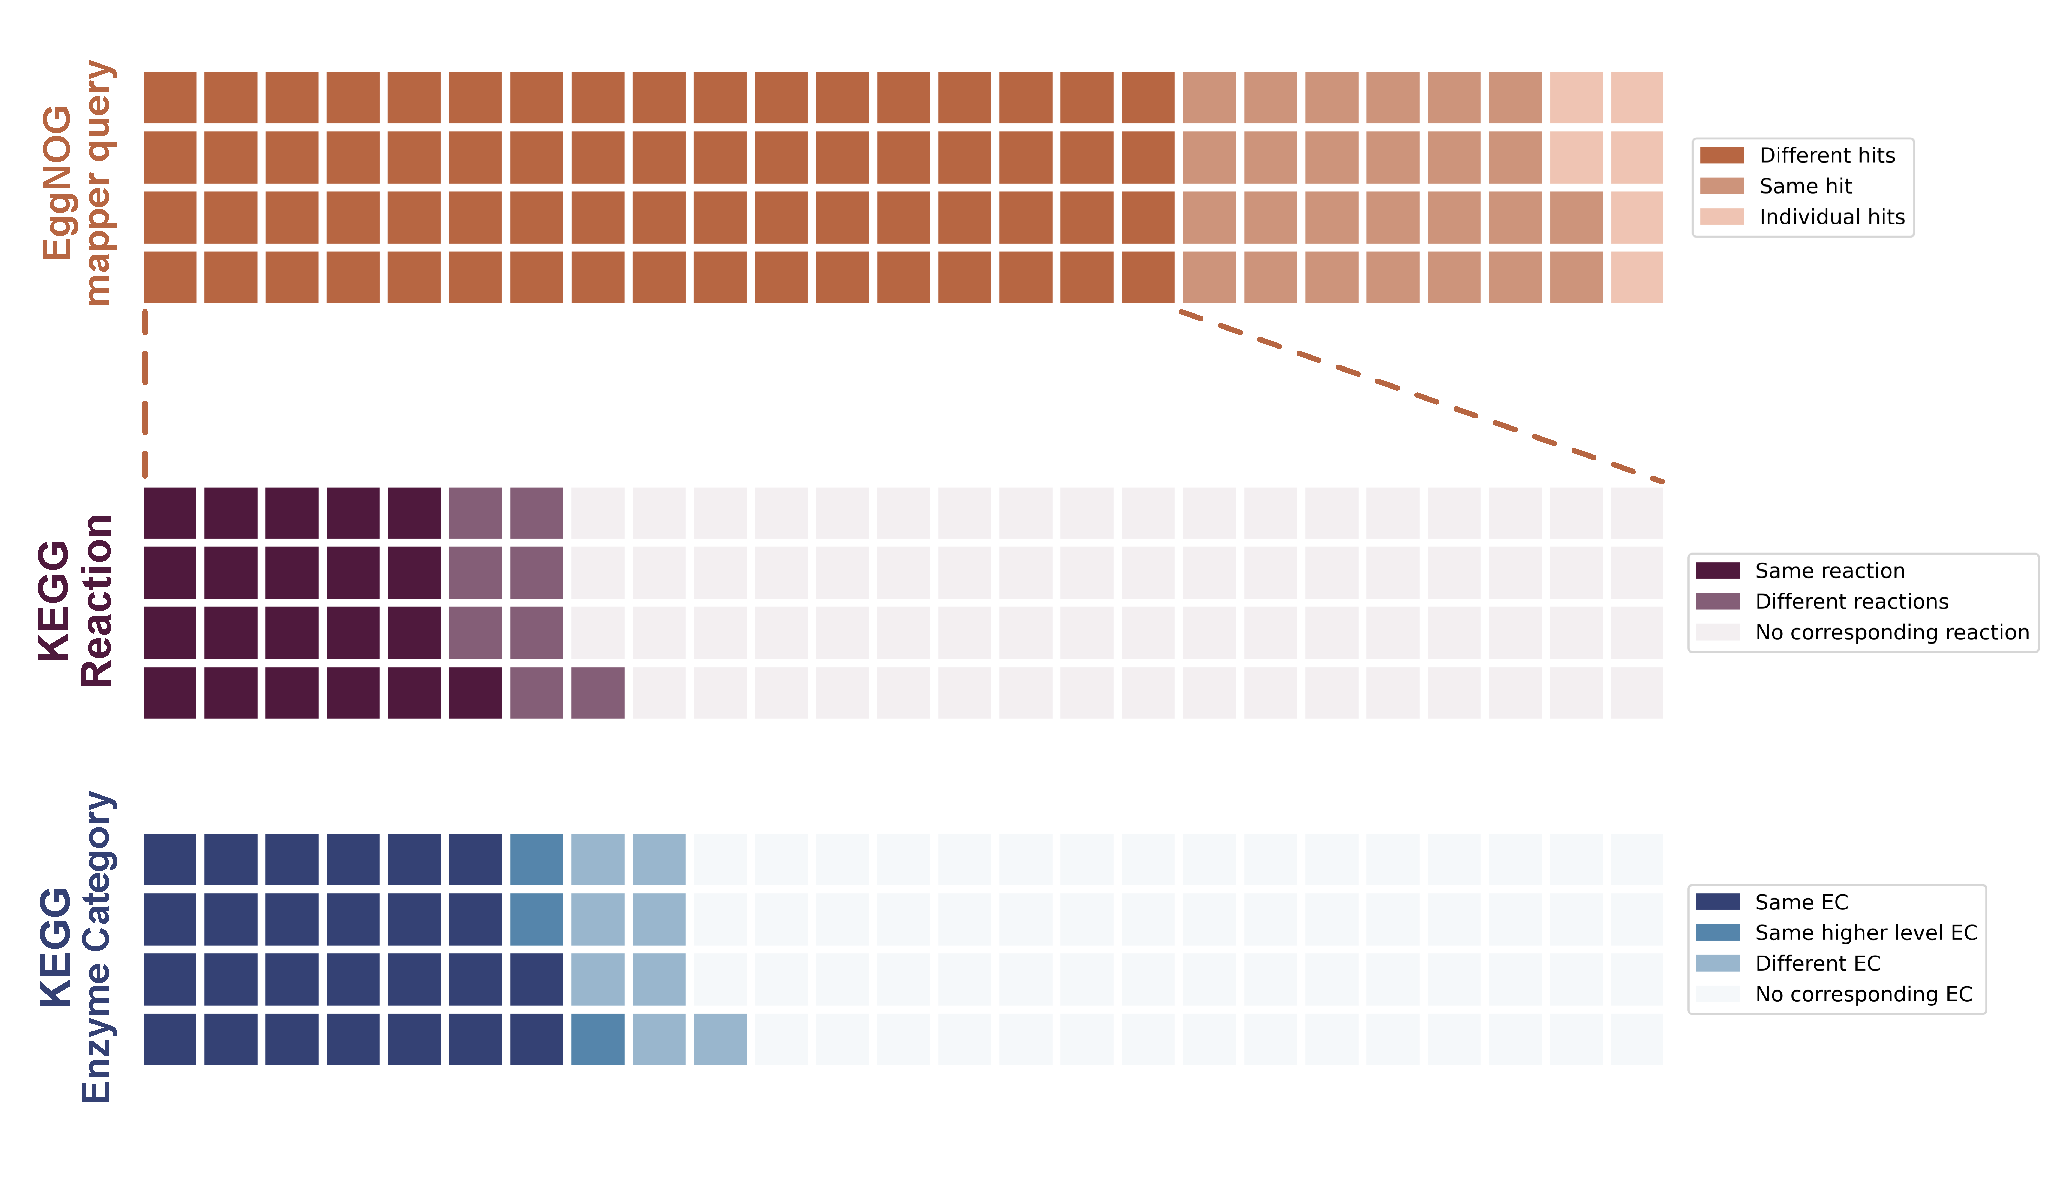
\includegraphics[width=0.95\textwidth]{waffleplot.pdf}
    \caption{Comparison of functional annotations between the first and medoid sequence of each ancestral Node zero (N0) for the archaea phylum level dataset. The waffle plot shows the percentage of a quantity---orange for number of OGs (used as a proxy for number of hits), purple for KEGG reaction number of different queries, and blue for KEGG enzyme commission (EC) number of different queries.  
    Every axis---orange, purple, and blue---shows a different statistic}
    \label{waffleplot}
\end{figure} 

From now on, we compare KEGG reaction and EC assignment only for the 68\% of eggNOG-mapper hits that differed between the first and medoid sequences. Most hits do not correspond to neither a reaction ID nor an EC number (Fig. \ref{waffleplot} gray blocks). Considering that the GTDB data used in our study only contain sequences predicted by Prodigal to be protein-coding, the absence of a match for the majority of the sequences is perplexing; it raises questions regarding the incompatibility between tools and databases used throughout the globe for genomic and metagenomic workflows. For hits that do find a match in the KEGG database, 73\% share the same KEGG reaction ID, and another 71\% share the same 4-digit EC number (Fig. \ref{waffleplot} purple and blue). With regard to the KEGG EC assignment, if we relax our constraints and compare EC assignments up to the third digit, which specifies the nature of the reaction \cite{mcdonald2009}, the percentage of shared EC assignments increases to 79\%. This simple statistical analysis stresses how important the choice of representative sequence is for functional annotation, even for related sequences that may have descended from the same gene.  

For our inferred ancestral genomes belonging to the archaea phylum and class level datasets, the medoid sequence was calculated from the full alignment and utilized for OG functional annotation. For the rest of the datasets (found in Table \ref{datasets}), we sampled a hundred sequences from each OG at random, and calculated the medoid only for those. Since the medoid is calculated by pairwise alignment of all sequences in an OG, the computational burden increases according to the Gauss's summation formula (Equation \ref{eq:alignments}), where \textit{n} is the number of sequences. As our datasets grow in size, the number of sequences attributed to each OG increases to a point where calculating the medoid becomes extremely time-consuming. For example, an OG with 1000 sequences---which becomes common in our larger datasets---would require 500,500 pairwise alignments. We therefore opted for a computationally tractable approach, calculating the medoid for a hundred randomly sampled sequences for OGs larger than that. Instead of calculating the medoid for all OGs, we could also have annotated all sequences of an OG, and then choose the most common eggNOG OG (eggNOG orthogroup) or COG (cluster of orthologous genes) category as the representative one for the OG, as done by Xavier et al. \cite{xavier2021}. 

\begin{equation}
    \label{eq:alignments}
    \sum_{i=1}^{n} i = \frac{n(n+1)}{2}
\end{equation}

As mentioned above, functional annotation does not only depend on the sequence itself, but on the database against which it is aligned. A feature of eggNOG-mapper version 2 \cite{cantalapiedra2021} allows for the generation of taxon-specific eggNOG databases. We therefore generated three databases spanning the prokaryotic domain, one for the Archaea (2157), one for Bacteria (2), and a general one including both domains (2157, 2). We then performed functional annotation of genes predicted to be present for certain internal tree nodes (presented in Figure \ref{node_descendants_genomesize}) against the domain-specific and the general eggNOG databases, chose for the best hit between the two runs, as described in the Methods section, and reconstructed each metabolic network based on the KEGG reaction IDs assigned by eggNOG-mapper for each best hit. Extant genomes were annotated only against the general eggNOG database. 

We also tried performing functional annotation of entire OGs, instead of single protein sequences, with profile hidden markov models (HMMs), as a more sensitive, probabilistic approach. Profiles are position-specific scoring models that take into account conservation patterns specific to each sequence \cite{mount2009, gribskov1987}. Consequently, they can offer enhanced alignment and functional annotation quality. This methodology, however, is even more time-consuming than simply calculating the medoid, and was not feasible with our current computational resources. In future analyses, we plan to use HMMs for functional annotation of the OGs, and compare the results with those obtained by the medoid method.

\subsection*{Metabolism Reconstruction}
\addcontentsline{toc}{subsection}{Metabolism Reconstruction}


One of the first things we noticed when mapping our inferred reaction IDs to the KEGG database was the absence of multiple IDs per dataset and often incomplete or missing fields, leading to inconsistent information between reactions; for example, some reactions include the KEGG module or pathway, while others do not. Even though the KEGG databases provide a valuable resource for the field of bioinformatics and metabolism modeling \cite{kanehisa2000}, KEGG was primarily designed for visualization purposes, with its reactions often unbalanced \cite{wrzodek2013}, and even elementally inconsistent \cite{goldford2024}. For these reasons, we utilized the database compiled by Goldford et al. (2024) \cite{goldford2024}, which extends the KEGG reactions database by adding detailed organic and inorganic cofactor dependencies from various other databases, while excluding elementally inconsistent reactions. Reaction directionality was performed with eQuilibrator \cite{beber2022}, to ensure a more realistic network reconstruction.

To inspect the connectivity of the reconstructed metabolisms of putative, ancient microorganisms, we visualized the networks using iPath \cite{darzi2018}, an interactive metabolic pathway explorer that is based on four KEGG global maps. The hypothetical, genome-scale metabolic model of LACA for the family-level archaea dataset can be seen in Figure \ref{fam4arc_metnet}, while the rest of LACA-inferred metabolic networks can be found in Appendix Figs. \ref{phy4arc_metnet} - \ref{gen4arc_metnet}. Even at the phylum-level, the network seems relatively well-connected, with isolated reactions being dispersed across the entire map.

\begin{figure}[H]
    \centering
    \includegraphics[width=0.98\textwidth]{metabolism/fam_arc_N0.pdf}
    \caption{Reconstruction of LACA's metabolic network from extant life, for the family-level archaea dataset. In black: enzymes and metabolic pathways that were inferred to be present in LACA.}    
    \label{fam4arc_metnet}
\end{figure}

%Another drawback of using KEGG Orthology (KOs), instead of COGs---which correspond to wider gene families---\cite{tatusov2003}, to construct hypothetical metabolism models of ancient microorganisms, is that gene families that were likely present in those organisms are divided into multiple KO families that appear in particular taxonomic groups and may only be inferred for younger ancestors \cite{moody2024}.

Phylogenetic-based metabolic network reconstruction enables the mapping of genetic information to genome distance from the tree root. We aimed to explore the emergence and evolution of individual ECs across the tree of life (ToL), a topic that has not been previously investigated. For this, we acquired the distance of all nodes from the tree root and used it as a proxy for evolution.

All enzyme categories are present in the reconstructed LACA metabolism (Figure \ref{ec_vs_rootdist_fam}B). The relative abundance of ligases and oxidoreductases is higher in the inferred ancient metabolisms, while that of transferases declines. Lyases and isomerases are universally more limited and do not become enriched over time. This divergence may indicate a different rate of innovation for various ECs or suggest that specific types of enzymes are more prone to either loss or gain.

\begin{figure}[H]
    \centering
    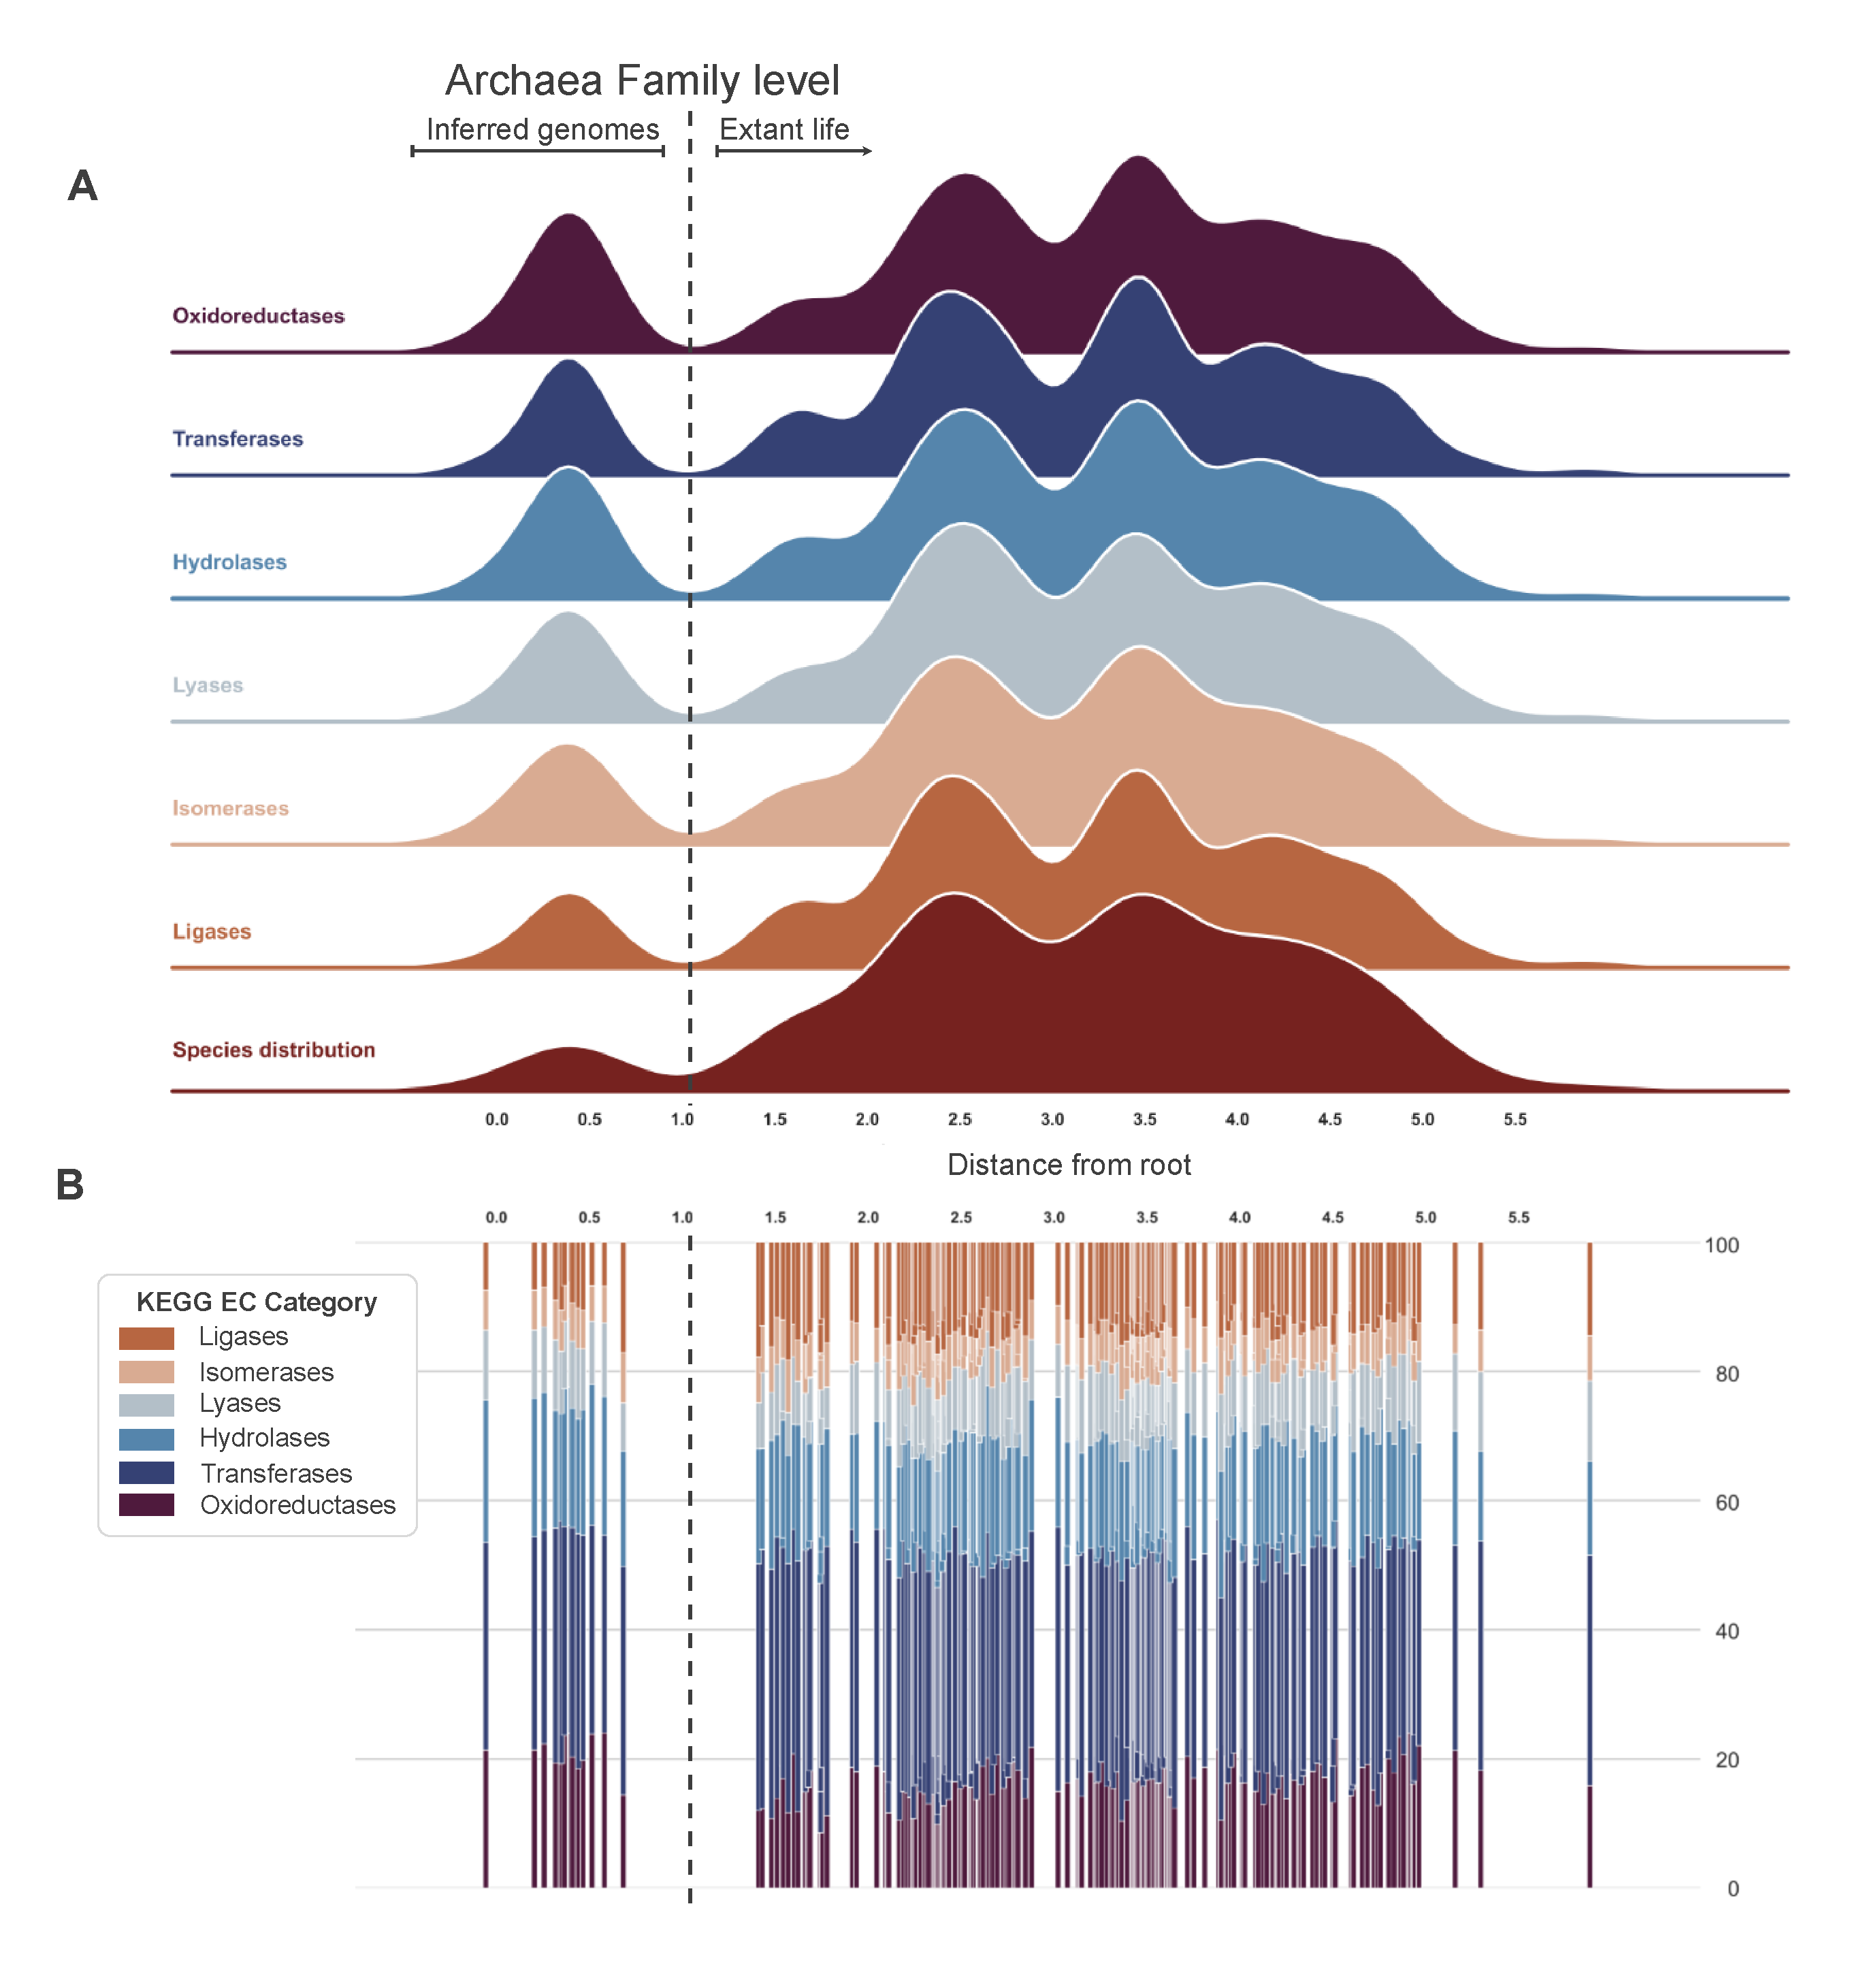
\includegraphics[width=0.9\textwidth]{ridgeplots/ec_vs_rootdist_fam.pdf}
    \caption{Evolution of individual enzyme categories for the family-level archaea dataset. The dashed line separates the inferred ancient metabolisms, on the left, from the extant ones, on the right. The ridgeplot of panel (A) displays the distribution of each category as a function of distance from the tree root, with the last axis presenting the species distribution. (B) shows the relative abundance of each category at that particular distance as a stacked barplot.}
    \label{ec_vs_rootdist_fam}
\end{figure}  

No other significant differences or patterns are observable, so it may be beneficial to divide the tree into multiple clades and track EC evolution within specific groups of species rather than across the entire tree. This approach will be especially important if we increase the deep branch resolution by reconstructing the metabolic networks of all possible internal tree nodes. Even though the relative abundance of the six EC categories varies between inferred and extant microorganisms, their distribution across the tree follows a similar pattern, reflecting the species distribution across the tree (Fig. \ref{ec_vs_rootdist_fam}A). 

Small variations, such as the relative decrease in transferases at a distance of around 2.0 from the tree root, may indicate an enrichment of this enzyme category in certain species. This could be due to specialization or an evolutionary advantage. The evolution of ECs across the ToL for the rest of the archaeal datasets can be found in Appendix Figures \ref{barplot_phy4arc} - \ref{barplot_gen4arc}.



\subsection*{Metabolic Network Expansion}
\addcontentsline{toc}{subsection}{Metabolic Network Expansion}

One of the first objectives of this internship was to investigate the evolution of metabolism across the ToL, and the metabolic potential of the inferred ancient microorganisms, with Metabolic Network Expansion (MNE). MNE is a graph-based structural analysis of large-scale metabolic systems \cite{ebenhoh2004}, that has previously been used to explore the metabolic scope of extant microorganisms. While the method itself does not take into account the phylogenetic relationships between species, Handorf et al. \cite{handorf2005}, among others, have noted that it exhibits evolution-like features. The sequential order of reaction addition to the expanding network, however, depends solely on the nature, and thus topology, of the seed compounds used to initiate the expansion. Therefore, it can be described as pre-determined.

For example, Figure \ref{fam4arc_metnetexp_0106} shows the expansion of the family-level LACA for two different seed sets: the one with the lowest 10\% complexity compounds based on the Bertz complexity index (A) and the one with the lowest 60\% complexity compounds (B); the respective seed set sizes can be found in Table \ref{seedset_sizes}. Appendix Figure \ref{fam4arc_metnetexp_1} provides further insight by visualizing the network expansion using the 100\% complexity seed set.

The 10\% seed set expansion is more limited, with fewer seed compounds (red dots) that are unevenly distributed throughout the metabolic map. Different parts of the metabolism will be accessed (gray lines) depending on the positions of the seeds, and the expansion will transpire with a specified order of reaction addition, since it is simulated as an iterative process. A visual representation like the one above quickly reveals the pre-determined nature of MNE. If anything, MNE suggests the flow of information in the system more than it reveals evolution-like traits.

While the inclusion of more seed compounds leads to a more extensive network, the richness of the seed set and clustering of the seeds in specific map regions limit the expansion to a few iterations. The first iteration introduces the largest change in the network, and the total difference in numbers between the scope (blue dots) and seed (red dots) size is small. Additionally, since the seed sets are randomly generated based on the Goldford et al. (2024) \cite{goldford2024} Bertz complexity list, seeds fall in part outside the reconstructed network. This is illustrated in Figure \ref{fam4arc_metnetexp_0106}, and more clearly in Appendix Figure \ref{fam4arc_metnet_plus_seedset}, where several red dots representing the seed compounds are disconnected from any of the black lines that denote the network reactions. The seed set size used for expansion will therefore always be equal to or smaller than the initially generated seed set size, so the ratio of the two will range between 0 and 1. We use this ratio instead of the initial or expansion-used seed set sizes in our MNE statistical analysis.

\begin{figure}[H]
    \centering
    \includegraphics[width=0.98\textwidth]{metabolism/fam_N0_exp0106_comp.pdf}
    \caption{Reconstruction of LACA's metabolic network from extant life, for the family-level archaea dataset. In black: enzymes and metabolic pathways that were inferred to be present in LACA, which are not part of the expansion. In gray: enzymes and metabolic pathways of the expanded network. Red dots: respective seed set compounds. Blue dots: scope compounds after network expansion. (A) shows the expansion of the network with the 10\% completeness seed set, while (B) shows the expansion with the 60\% completeness seed set.}    
    \label{fam4arc_metnetexp_0106}
\end{figure}

A straightforward way to compensate for this lack of overlap between the seed set and the reconstructed metabolic network, while increasing the spread of the seeds in the network is to select a set number of compounds from each KEGG module. However, it may be more beneficial to manually select prebiotic or at least lower complexity compounds from a variety of molecular classes. In this way, the seeds will be more evenly distributed throughout the network, and the expansion will be more extensive, potentially with more iterations.



\begin{wraptable}{l}{0.4\textwidth}
    \caption{Seed set initial sizes.}
    \begin{tabular}{lc}

        \textbf{Seed set} & \textbf{Seed set size} \\ \hline\hline
        \addlinespace[0.5ex]
        Standard & 70 \\ 
        Meteorite Soup & 81 \\ 
        Spark Discharge & 99 \\ 
        10\% Complexity & 160 \\ 
        20\% Complexity & 270 \\ 
        40\% Complexity & 487 \\ 
        60\% Complexity & 683 \\ 
        80\% Complexity & 931 \\ 
        100\% Complexity\footnotemark & 1183 \\ 
        \bottomrule
    
    \end{tabular}
    \label{seedset_sizes}
\end{wraptable}

\footnotetext{The complexity seed sets originate in the Bertz complexity index list of Goldford et al. (2024) \cite{goldford2024} Supplementary Table S6. The generation of the seed sets is described in the Methods section.}

\normalsize
For a given seed set, the seed set size ratio increases rapidly with smaller genome sizes but soon reaches a plateau (Fig. \ref{overview_ancient}A). As demonstrated in Figures \ref{fam4arc_metnet} and \ref{phy4arc_metnet} - \ref{gen4arc_metnet}, the reconstructed metabolic networks of LACA across various taxonomic levels show minimal variation, despite substantial increases in genome size for the respective LACA genomes. The saturation curve suggests that the metabolic network size stabilizes once a certain genome size is reached, indicating that the maximum number of enzymes present in the inferred genomes and available for inclusion in the network has been attained. This is also reflected in the median genome and metabolic network sizes of hypothetical ancient microorganisms: 8222 protein-encoding genes, and 1514 enzymes, respectively.

For the various seed sets, the seed set size ratio decreases as the total seed set size increases (Fig. \ref{overview_ancient}A), implying that compounds of higher complexity are progressively less integrated into the expansion. In other words, the larger the seed set, the more seeds fall outside the reconstructed network and are never utilized in the expansion.

Both the seed set size and scope size (Fig. \ref{overview_ancient}B) of an expansion exhibit similar behavior with genome size increase, reaching a plateau after a certain threshold. This is demonstrated by their linear relationship (Fig. \ref{overview_ancient}C), with the exception of the \textit{spark-discharge} seed set, suggesting that the expansion is proportional to the seed set rather than the genome size.

The scope size distribution for the inferred, ancient metabolisms (Fig. \ref{overview_ancient}D) appears to fall into two distinct categories, divided largely by the seed set size: symmetrical and bimodal. Smaller seed sets that do not initiate expansion, regardless of genome size, produce a single prominent peak around the median scope size, with values distributed symmetrically on both sides. The \textit{spark-discharge} seed set (available along all other seed sets at the data/seedsets folder in \href{https://github.com/astrademertzi/metnetexp_report}{this} github repository), which includes 11 L-amino acids, is the only of the smaller-size seed sets for which the ratio does not correlate linearly with scope size (Fig. \ref{overview_ancient}C); better-integrated seed sets seem to also allow for larger expansions, resulting in a largely skewed bimodal distribution. This behavior can be seen more clearly in Appendix Figure \ref{gfsd_scopesize}, where only a few ancient reconstructed metabolic networks are able to provide larger scopes. %Expansion begins with the \textit{20\% complexity} seed set, and the scope size follows a bimodal distribution, largely symmetrical around the median, with the lower-value peak being slightly wider. 

One last trend worth mentioning is the large comparative increase in scope size when transitioning from the \textit{40\% complexity} to the \textit{60\% complexity} seed set (see Figures \ref{overview_ancient}D and \ref{overview_extant}D). This transition may give an indication about the relative number of compounds a microorganism may need to acquire from the environment to sustain its metabolism (around 600, as shown in Table \ref{seedset_sizes}), but a much better approach to investigate this would be to explore the \textit{minimal} seed sets of the reconstructed networks.


According to Handorf et al. (2008) \cite{handorf2008}, the minimal seed set of an entire metabolic network is the smallest set of compounds capable of producing all its metabolites. This approach has shown that minimal seed sets reflect the nutritional requirements of the microorganisms under analysis. In a reverse ecology concept, as Borenstein et al. (2008) \cite{borenstein2008} have demonstrated, this approach can predict the nutrients a microorganism can acquire from the environment. Therefore, when applied to the hypothetical reconstructed metabolisms of ancient microorganisms, this method could provide insights into the environmental conditions in which they could have thrived.

\begin{figure}[H]
    \centering
    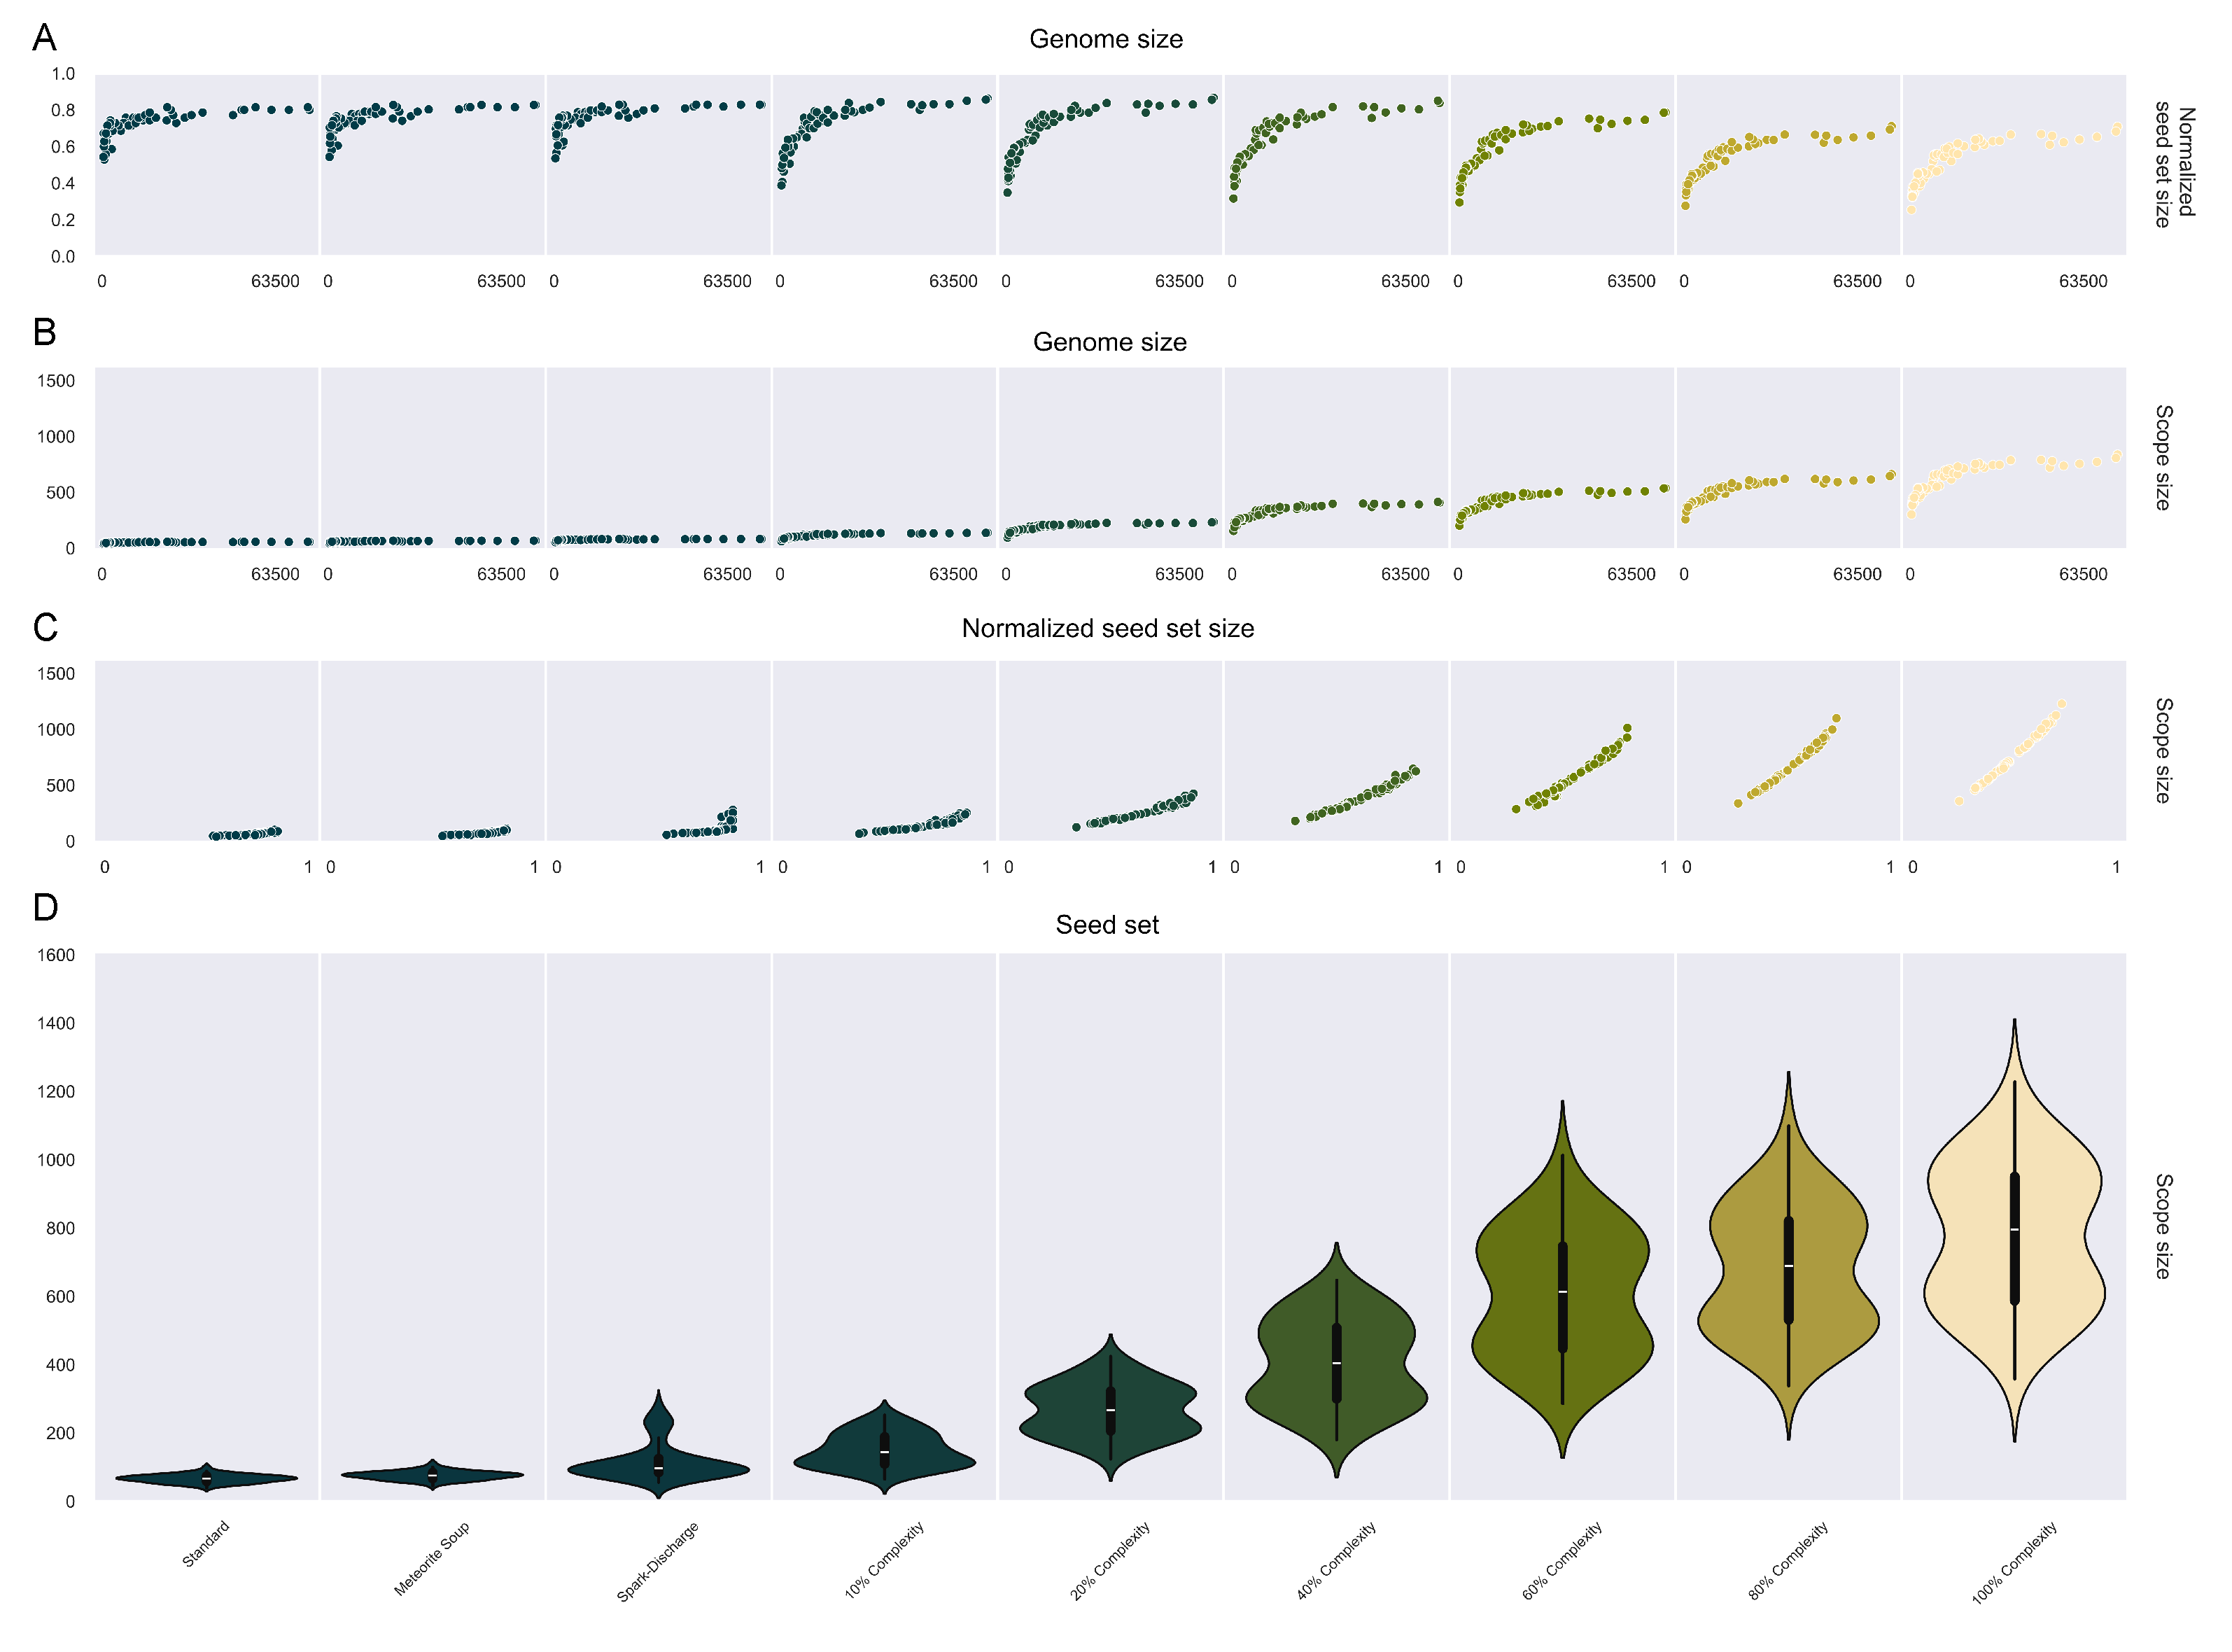
\includegraphics[width=0.98\textwidth]{overview_expansion/overview_ancient_final.pdf}
    \caption{Overview of the MNE for all inferred ancient metabolisms. (A) shows the microorganisms' inferred genome size as a function of the normalized seed set size for each seed set. The number of protein-encoding genes is used as a proxy for genome size, while the normalized seed set size reflects the number of seed compounds found in the network divided by the initial number of seeds. (B) displays scope size as a function of genome size for each seed set, with scope size defined as the number of compounds in the network after expansion. (C) illustrates the normalized seed set size as a function of scope size for each seed set. (D) presents the scope size distribution for each seed set in the form of a violin plot.}
    \label{overview_ancient}
\end{figure} 

The overview statistics for the MNE of extant microorganisms appear to follow similar trends, while demonstrating a few stark differences (Fig. \ref{overview_extant}). It is immediately apparent that the maximum scope size for extant genomes is smaller than that for ancient ones. Moreover, the symmetrical bimodality of the scope size distribution seen for larger seed sets in ancient genomes is replaced by a skewed one towards smaller values. This behavior aligns with the fact that most extant microorganisms have smaller, more specialized metabolisms than those inferred by OF. The median genome size for extant prokaryotes is 2237 protein-encoding genes, whereas inferred genomes are 3.5 times that size on average. In terms of metabolic network size, extant microorganisms average 878 enzymes, covering approximately 40\% of their genome size, while inferred ancient microorganisms have a median metabolic network size of 1514 enzymes, 1.7 times larger than that of extant ones, accounting for about 20\% of their genome size. Comparing that to the maximum size of an extant metabolic network, which is 1892 enzymes, underscores the biosphere-level nature of the inferred ancient metabolisms, and may hint at the universal metabolic core of extant life. An alternative, simplified approach that could provide further insight into this hypothesis would be to isolate the highly shared genes among all extant microorganisms and compare their reconstructed metabolic networks with those inferred using the DLC model in the current study.

\begin{figure}[htpb]
    \centering
    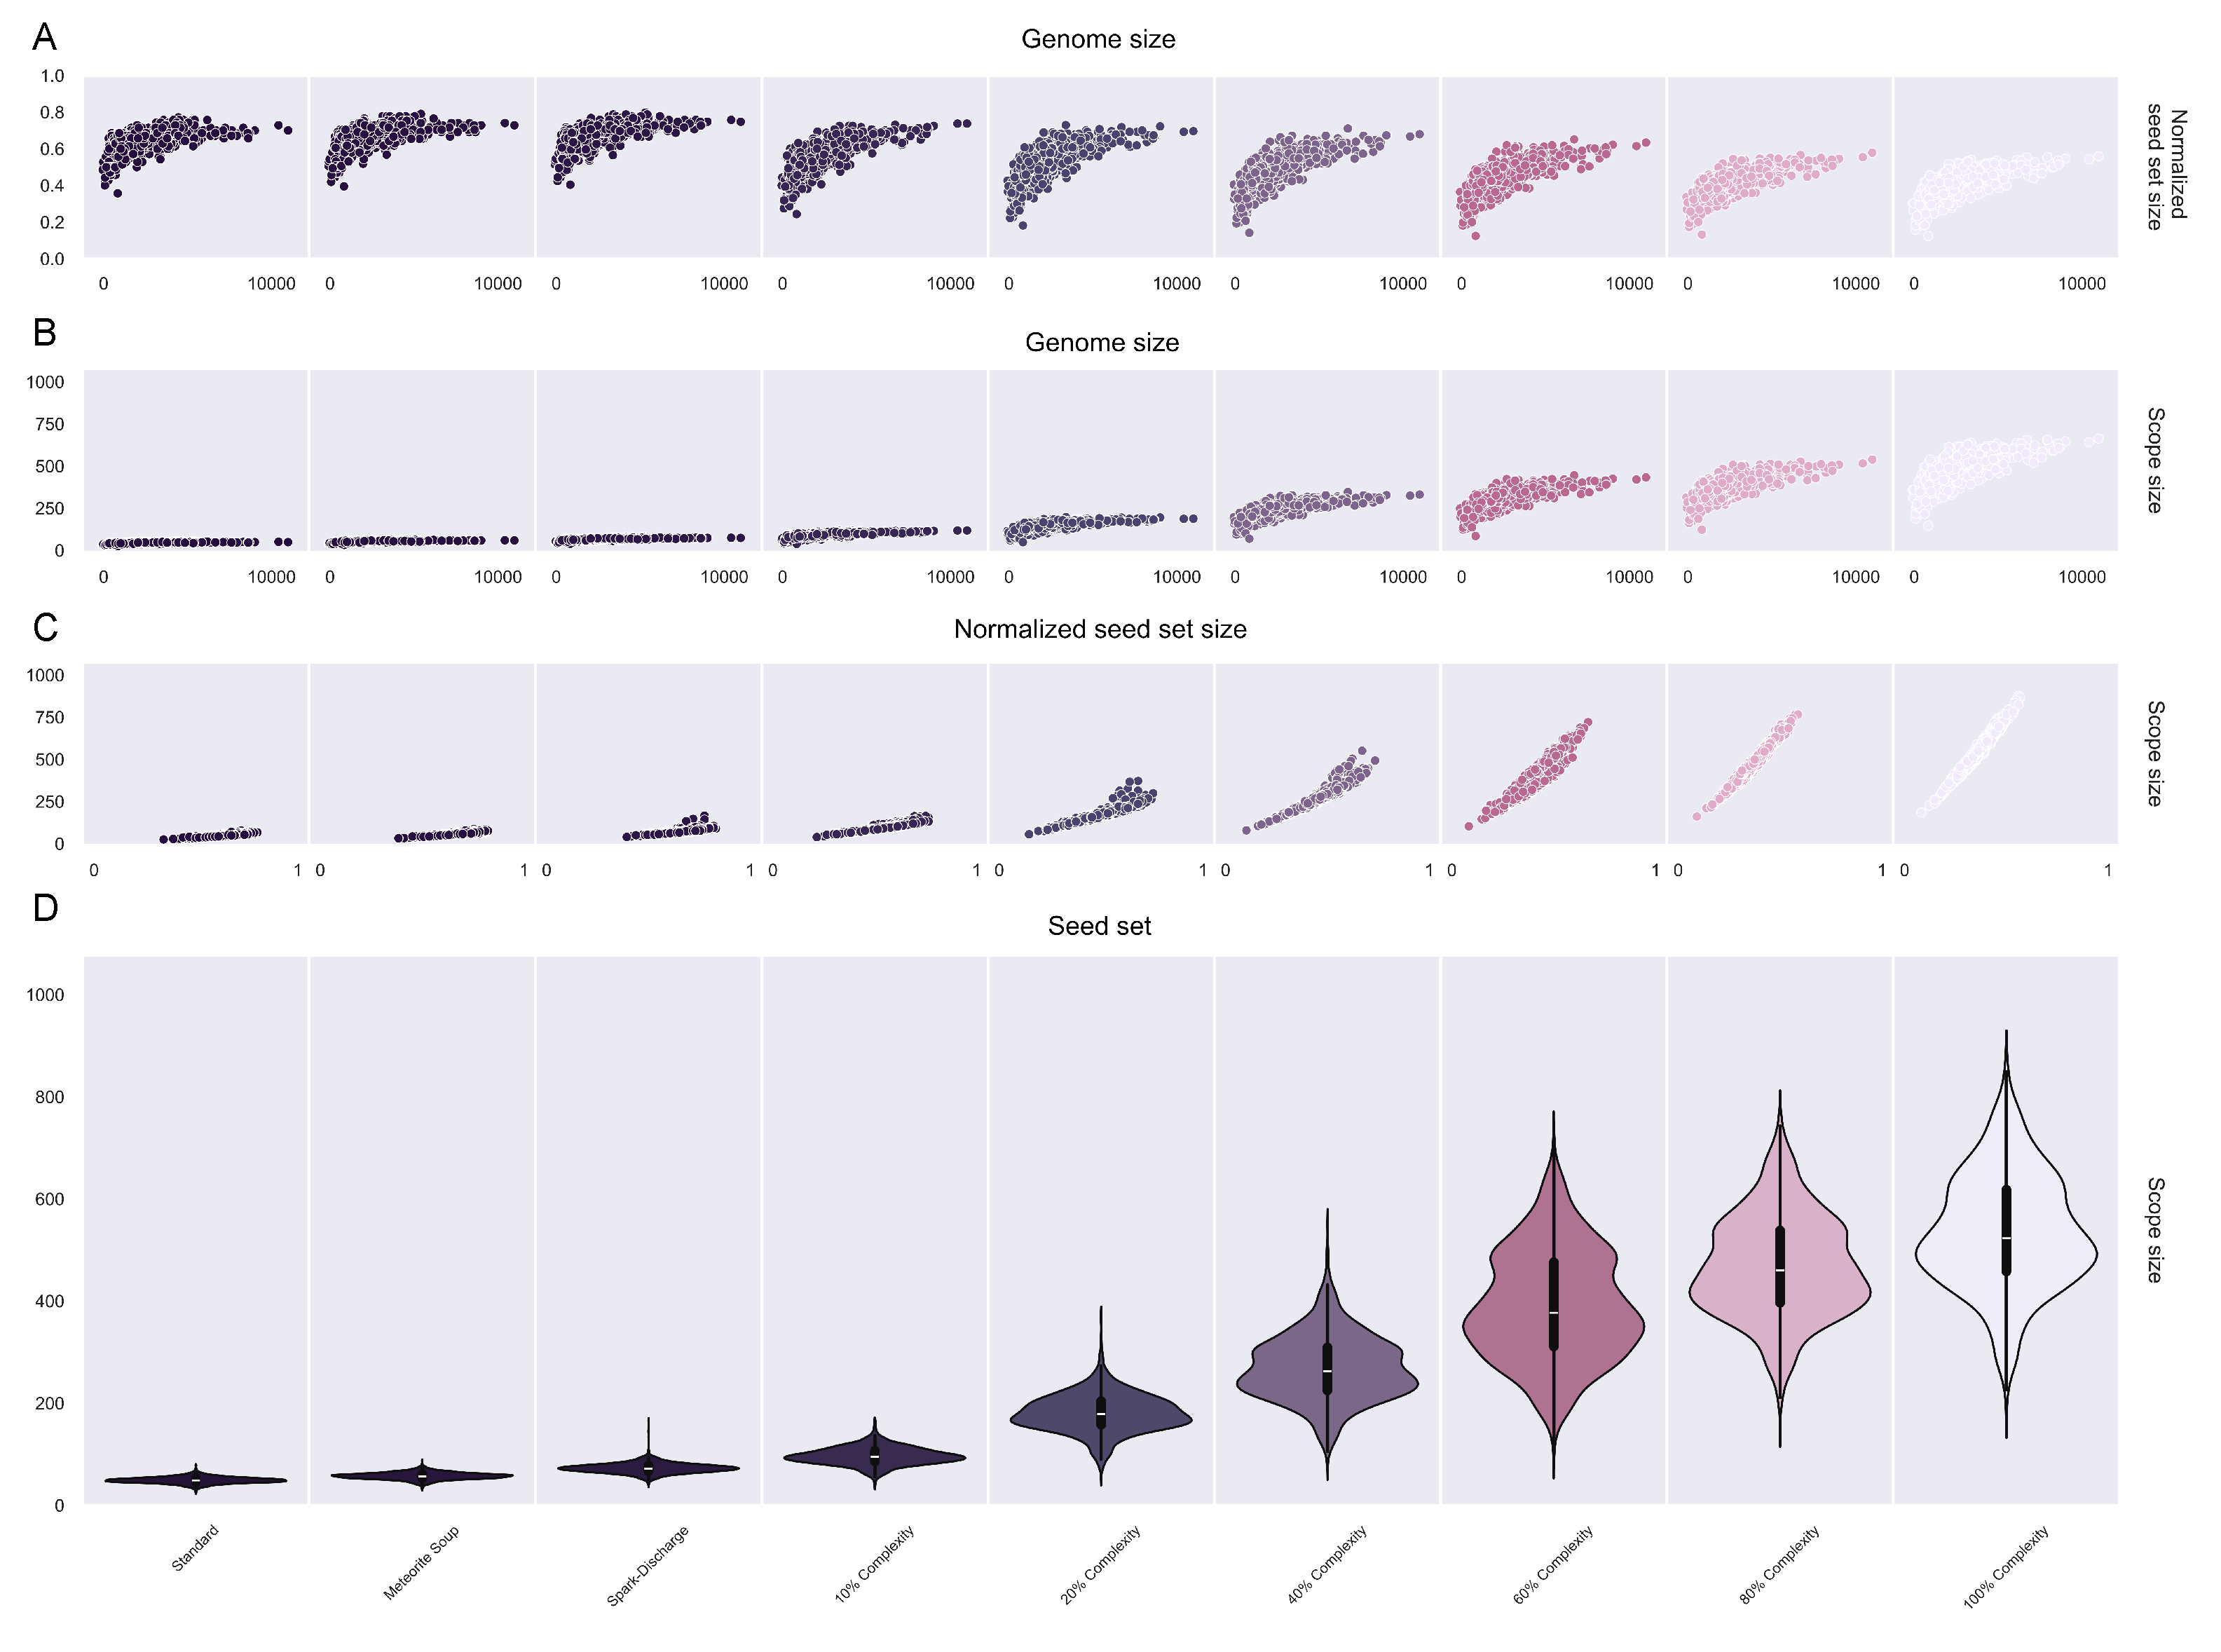
\includegraphics[width=0.98\textwidth]{overview_expansion/overview_extant_final.pdf}
    \caption{Overview of the MNE for all extant metabolisms. (A) shows the microorganisms' inferred genome size as a function of the normalized seed set size for each seed set. The number of protein-encoding genes is used as a proxy for genome size, while the normalized seed set size reflects the number of seed compounds found in the network divided by the initial number of seeds. (B) displays scope size as a function of genome size for each seed set, with scope size defined as the number of compounds in the network after expansion. (C) illustrates the normalized seed set size as a function of scope size for each seed set. (D) presents the scope size distribution for each seed set in the form of a violin plot.}
    \label{overview_extant}
\end{figure}   

Unlike ancient metabolic networks, where seed set size follows a linear relationship with scope size, extant networks exhibit a more complex behavior, particularly for medium-sized and medium-complexity seed sets. There appears to be a split at higher seed set integration rates, resulting in distinct but not significantly different scope sizes. While there is a slight correlation between scope and genome size, the observed split likely relates to which seeds are integrated into the extant reconstructed network, their distribution on the metabolic map, and the network's structure. This behavior highlights the metabolic diversity and specialization of extant microorganisms, and the importance of the seed set nature in determining the network's expansion.


\section{Conclusions \& Outlook}
\normalsize

To this author's knowledge, this research project is the first to explore the expansion of metabolic networks constrained by phylogenetic relationships, and to investigate the effect of taxon sampling on ancient genome inference. 

Phylogenetic analyses appear robust to random taxon sampling at the same dataset size, as demonstrated by performing separate OF analyses on triplicate datasets for the archaea phylum and class levels. While including more species can better capture the evolutionary relationships between genes and gene families, it does not necessarily enhance species tree accuracy, as previously stated \cite{martinez-gutierrez2021}. These results suggest that depending on the research question, the inclusion of more species may be beneficial. For instance, studies aiming to define Archaeal or Bacterial Tree topologies will benefit from more limited taxon sampling, while studies like this one need broader sampling to capture the full extent of prokaryotic diversity. 

Results can vary significantly depending on both taxon sampling and the evolutionary model used for ancient gene content inference. Unlike previous research, which has investigated the physiology and metabolic potential of prokaryotic ancestors such as LUCA, LACA, and LBCA, we have employed a different parsimonious evolutionary model, the DLC model. This model does not account for horizontal gene transfer, which is integral to prokaryotic life. Consequently, the inferred genome sizes correlate positively with the number of species included in the analysis, with ancient gene content being multiple times larger than the average extant genome for any given dataset of the analysis. The DLC model, however, remains relevant. By shifting focus from the hypothesis that a single microorganism gave rise to all extant diversity to the possibility that a pool of microorganisms from the ancient biosphere evolved into modern life, the DLC model can provide valuable insights into the core metabolic functions of extant life.

Regarding the reconstruction of both extant and ancient metabolic networks using eggNOG-mapper, a gold standard and state-of-the-art tool for gene functional annotation, we found that a portion of annotated genes expected to be assigned a KEGG function were not assigned one. This finding underscores two points of interest in bioinformatics research: the discrepancy of gene family clustering algorithms and function assignment (KOs, COGs, eggNOGs) between the various tools and databases used in genomic and metagenomic workflows, and the need for transitioning to a more comprehensive database than KEGG for metabolic modeling. 

As far as the evolution of metabolism is concerned, conclusions are less concrete. The current analysis points to the existence of all six enzyme categories in the ancient biosphere. Their relative abundance, however, was probably different to that of extant life.

Performing metabolic network expansion with various seed sets across the extant and extinct parts of the tree of life challenges the previously held view that this process reflects evolution-like traits. We show that the expansion depends on the nature, topology, and number of seeds used for expansion, and echos the flow of chemical information within the network. Different seeds will yield differentially expanded networks, which highlights the importance of nutrient availability for proper metabolic function. 

The future of this research project is full of exciting possibilities. An important development is the creation of a \textit{'poor species detection'} algorithm. This tool will automate the identification of genetically underrepresented species in a dataset and enable the gradual integration of new closely-related taxa. The aim is to improve initially poor taxon sampling over time, while keeping the dataset size minimal, making the process both time- and cost-effective. This approach may also estimate under-sampled species in the tree of life, facilitating future sampling efforts.

Another potential improvement lies in the evolutionary analysis of metabolism we have performed. Instead of analyzing EC evolution across the tree of life, it will be more informative to focus on enzyme evolution within specific clades. This approach will allow for a more detailed understanding of the evolution of metabolic pathways for specific groups of microorganisms with specialized metabolisms, such as methanogens, halophiles, or thermophiles. Moreover, since no single species tree topology can be considered the \textit{one, true topology}---phylogenetics approaches are, after all, probabilistic---exploring ancient gene content under various tree topologies would be very interesting. Comparing the inferred gene contents and identifying the most commonly shared functionalities may even provide a more representative estimation of the core gene content for both extant and ancient life.

The current study has only scratched the surface of what is possible with regard to metabolic network expansion. A very useful extension of the analysis would be to use MNE to quantify a system's metabolic potential based on metabolite availability in the environment, essentially by developing a metric to measure expansion. Since our current, randomly generated seed sets are sometimes poorly integrated into the reconstructed metabolic networks, it would be beneficial to create manually curated seed sets of comparable size and complexity. This would allow for a more detailed investigation of the flow of chemical information within specific networks of interest. 

The most valuable addition to the MNE analysis would be integrating the minimal seed set approach. This method would help identify the nutritional requirements of putative ancient microorganisms and provide insights into the environmental conditions they may have inhabited.

Despite its exploratory nature, this project provides valuable insights into the challenges of modern phylogenetics and introduces a new perspective on the nature of MNE. Overall, these observations underscore the importance of delving deeper into the data, questioning it, and maintaining an open mind when investigating the deepest branches of the tree of life.